\chapter{Analysis of Assignment Structures}

\section{Overview of Assignment Structures}

This assignment considers two structural systems to evaluate the performance of the developed analysis program under different loading conditions.

Structure (a) is a mixed frame--truss system subjected to support settlement. The response is driven entirely by prescribed displacements, providing a benchmark for verifying the implementation of stiffness matrix partitioning and reaction recovery.

Structure (b) is a frame--truss system subjected to thermal loading. The problem involves both uniform and gradient temperature effects, allowing verification of the thermal load formulation through equivalent nodal forces and fixed-end actions.

Together, these two cases cover the key extensions introduced in this assignment, namely support settlement and thermal loading, and provide a comprehensive validation of the solver for linear static analysis of combined frame and truss structures.

\section{Structure (a): Settlement Case}

\subsection{Model Description}

\begin{figure}[H]
\centering
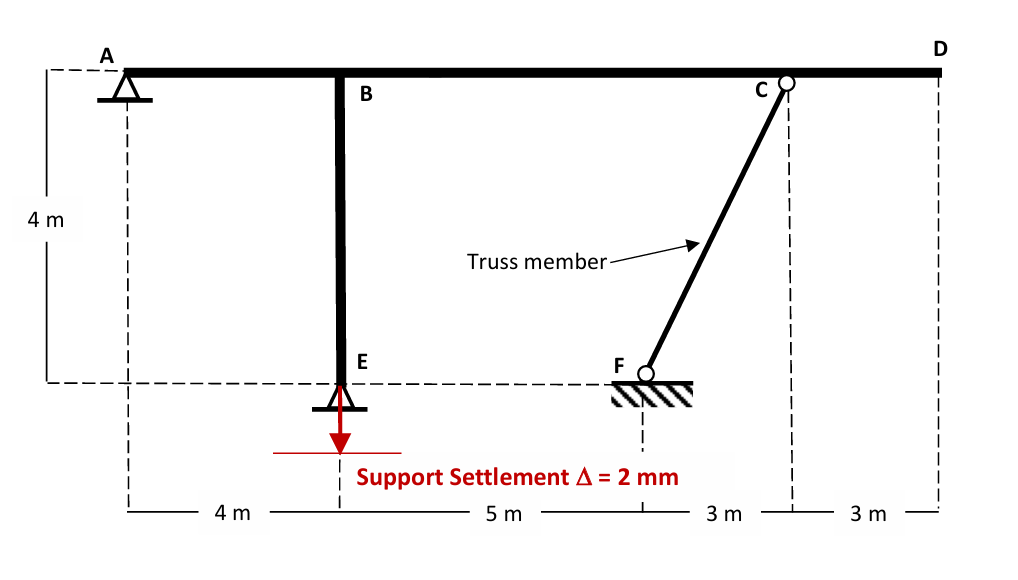
\includegraphics[width=0.85\textwidth]{ModelA.png}
\caption{Model of Structure (a): Settlement Case (Case 2a)}
\label{fig:case2a_model}
\end{figure}

Structure (a) consists of a concrete frame $ABCD$, a concrete column $BE$, and a steel truss member $FC$. The upper beam line extends from node $A$ to node $D$, with intermediate joints at $B$ and $C$. The column $BE$ connects node $B$ to the lower support at $E$, while the steel truss member $FC$ connects the ground support at $F$ to node $C$.

The geometry used in the benchmark model is:
\begin{itemize}
    \item $A = (0,4)\ \text{m}$
    \item $B = (4,4)\ \text{m}$
    \item $C = (12,4)\ \text{m}$
    \item $D = (15,4)\ \text{m}$
    \item $E = (4,0)\ \text{m}$
    \item $F = (9,0)\ \text{m}$
\end{itemize}

Members $AB$, $BC$, $CD$, and $BE$ are concrete frame members with 
\[
E = 3.0\times10^7\ \text{kN/m}^2
\]
and a $50\ \text{cm} \times 50\ \text{cm}$ square section. Member $FC$ is a steel truss member with
\[
E = 2.0\times10^8\ \text{kN/m}^2
\]
and pipe section properties corresponding to a $3\ \text{cm}$ outer diameter and $1\ \text{mm}$ wall thickness.

The loading is purely kinematic: node $E$ is subjected to a prescribed vertical settlement of
\[
u_y = -0.002\ \text{m}
\]
while no external mechanical loads are applied.



\subsection{Input Assumptions}

The following assumptions were adopted:

\begin{enumerate}
    \item The system is modeled as a two-dimensional linear elastic frame--truss system.
    \item Concrete members ($AB$, $BC$, $CD$, $BE$) are modeled as frame elements carrying axial force, shear force, and bending moment.
    \item Member $FC$ is modeled as a truss element carrying axial force only.
    \item The support settlement is imposed at node $E$ as a prescribed displacement $u_y = -0.002$ m.
    \item No external loads are applied; the response is entirely due to settlement.
    \item The truss member $FC$ is modeled as a diagonal member between $F(9,0)$ and $C(12,4)$.
\end{enumerate}

\subsection{Solver Results}

\subsubsection{Nodal Displacements}

\begin{table}[H]
\centering
\caption{Nodal Displacements}
\begin{tabular}{cccc}
\toprule
Node & $u_x$ (m) & $u_y$ (m) & $r_z$ (rad) \\
\midrule
A & 0.000000 & 0.000000 & $-6.607\times10^{-4}$ \\
B & $3.591\times10^{-6}$ & $-1.994\times10^{-3}$ & $-1.738\times10^{-4}$ \\
C & $5.368\times10^{-6}$ & $-9.569\times10^{-4}$ & $2.813\times10^{-4}$ \\
D & $5.368\times10^{-6}$ & $-1.129\times10^{-4}$ & $2.813\times10^{-4}$ \\
E & 0.000000 & $-2.000\times10^{-3}$ & $8.556\times10^{-5}$ \\
F & 0.000000 & 0.000000 & 0.000000 \\
\bottomrule
\end{tabular}
\end{table}

\subsubsection{Support Reactions}

\begin{table}[H]
\centering
\caption{Support Reactions}
\begin{tabular}{cccc}
\toprule
Support & $R_x$ (kN) & $R_y$ (kN) & $M_z$ (kN$\cdot$m) \\
\midrule
A & $-6.7323$ & $9.5105$ & 0.0000 \\
E & $5.0658$ & $-11.7330$ & 0.0000 \\
F & $1.6665$ & $2.2225$ & 0.0000 \\
\bottomrule
\end{tabular}
\end{table}

\subsubsection{Member-End Forces (Local Coordinates)}

\begin{table}[H]
\centering
\caption{Member-End Forces}
\begin{tabular}{cccccccc}
\toprule
Element & Type & $N_i$ & $V_i$ & $M_i$ & $N_j$ & $V_j$ & $M_j$ \\
\midrule
AB & Frame & $-6.7323$ & $9.5105$ & $0.0000$ & $6.7323$ & $-9.5105$ & $38.0420$ \\
BC & Frame & $-1.6665$ & $-2.2225$ & $-17.7789$ & $1.6665$ & $2.2225$ & $-6.98\times10^{-4}$ \\
CD & Frame & $0.0000$ & $0.0000$ & $0.0000$ & $0.0000$ & $0.0000$ & $0.0000$ \\
BE & Frame & $-11.7330$ & $-5.0658$ & $-20.2632$ & $11.7330$ & $5.0658$ & $0.0000$ \\
FC & Truss & $2.7779$ & $2.36\times10^{-4}$ & $4.82\times10^{-4}$ & $-2.7779$ & $-2.36\times10^{-4}$ & $6.98\times10^{-4}$ \\
\bottomrule
\end{tabular}
\end{table}

\subsection{Benchmark Comparison}

The solver results match the benchmark solution obtained from FTOOL to numerical precision. Key equilibrium checks are satisfied:

\[
\sum R_x = 0, \qquad \sum R_y = 0
\]

Element $CD$ carries zero internal force, while members $FC$ and $BC$ exhibit end moments and shears that are numerically negligible (on the order of $10^{-4}$ to $10^{-3}$), and may therefore be treated as zero for engineering purposes.

The small residual moment at the pinned end of member $BC$ ($\approx 10^{-4}$ kN$\cdot$m) is attributed to numerical precision and is considered negligible.

A comparison summary is given below:

\begin{table}[H]
\centering
\caption{Benchmark Comparison}
\begin{tabular}{cccc}
\toprule
Quantity & Solver & Benchmark & Difference \\
\midrule
$u_y(E)$ (m) & $-2.000\times10^{-3}$ & $-2.000\times10^{-3}$ & 0 \\
$R_x(A)$ (kN) & $-6.7323$ & $-6.7323$ & negligible \\
$R_y(E)$ (kN) & $-11.7330$ & $-11.7330$ & 0 \\
$N(FC)$ (kN) & $2.7779$ & $2.7779$ & negligible \\
$M_B(AB)$ (kN$\cdot$m) & $38.04$ & $38.04$ & negligible \\
\bottomrule
\end{tabular}
\end{table}

\begin{figure}[H]
\centering

\includegraphics[width=0.85\textwidth]{ModelA_Ftool.png}
\caption{FTOOL Benchmark Output for Structure (a)}
\label{fig:modelA_ftool}
\end{figure}

\section{Structure (b): Thermal Loading Case}

\subsection{Model Description}

Structure (b) consists of a concrete beam $ABC$ supported by steel truss members $BD$ and $BE$. The beam spans from node $A$ to node $C$ with an intermediate joint at $B$. The truss members connect node $B$ to supports at nodes $D$ and $E$.

\begin{figure}[H]
\centering
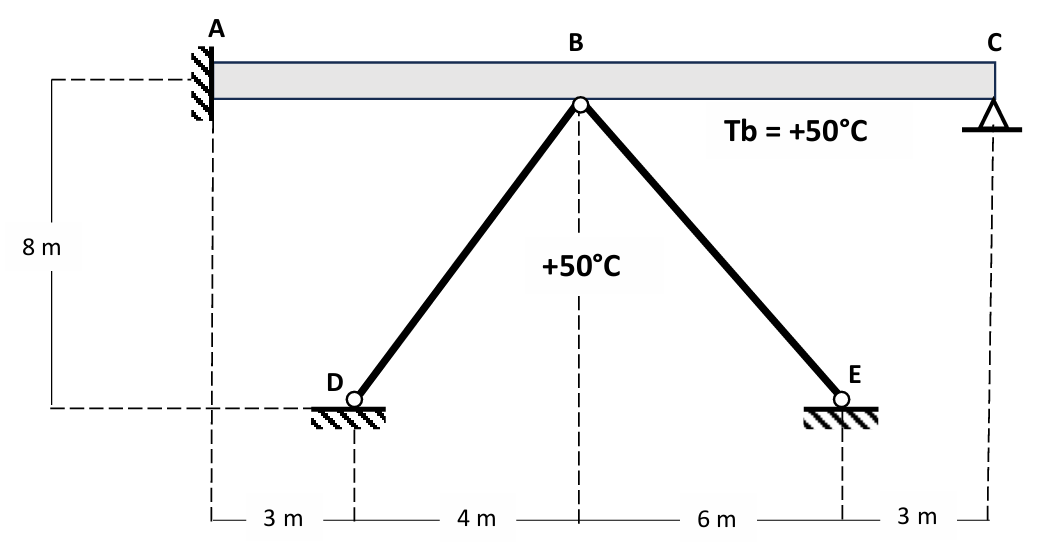
\includegraphics[width=0.85\textwidth]{ModelB.png}
\caption{Model of Structure (b): Thermal Loading Case (Case 2b)}
\label{fig:modelB_structure}
\end{figure}

The geometry used in the model is:
\begin{itemize}
    \item $A = (0,8)\ \text{m}$
    \item $B = (7,8)\ \text{m}$
    \item $C = (16,8)\ \text{m}$
    \item $D = (3,0)\ \text{m}$
    \item $E = (13,0)\ \text{m}$
\end{itemize}

The concrete beam $ABC$ has material properties:
\[
E_c = 3.0\times10^7\ \text{kN/m}^2, \quad \alpha_c = 8\times10^{-6}\ ^\circ\text{C}^{-1}
\]
with a rectangular section:
\[
b = 0.40\ \text{m}, \quad h = 0.80\ \text{m}, \quad 
A = 0.32\ \text{m}^2, \quad I = 0.01707\ \text{m}^4
\]

The steel truss members $BD$ and $BE$ have:
\[
E_s = 2.0\times10^8\ \text{kN/m}^2, \quad \alpha_s = 1.2\times10^{-5}\ ^\circ\text{C}^{-1}
\]
and pipe section properties corresponding to a $3\ \text{cm}$ diameter and $1\ \text{mm}$ thickness.

\subsection{Thermal Loading Definition}

The loading is purely thermal. According to the problem statement:

\begin{itemize}
    \item The bottom fiber of the concrete beam is heated by $+50^\circ$C
    \item The top fiber remains at $0^\circ$C
\end{itemize}

Thus, for frame elements:
\[
T_{\text{top}} = 0, \quad T_{\text{bottom}} = +50^\circ C
\]

The resulting thermal components are:
\[
T_{\text{mean}} = \frac{T_{\text{top}} + T_{\text{bottom}}}{2} = 25^\circ C
\]
\[
\Delta T_{\text{diff}} = T_{\text{bottom}} - T_{\text{top}} = 50^\circ C
\]

\subsubsection*{Thermal Gradient Sign Convention}

The local element coordinate system is defined with the $x$-axis along the member and the $y$-axis positive upward. The top fiber corresponds to positive $y$, and the bottom fiber corresponds to negative $y$.

\begin{itemize}
    \item $T_{\text{top}}$: temperature at $+y$
    \item $T_{\text{bottom}}$: temperature at $-y$
    \item $\Delta T_{\text{diff}} = T_{\text{bottom}} - T_{\text{top}}$
\end{itemize}

A positive $\Delta T_{\text{diff}}$ produces sagging curvature.

\begin{table}[H]
\centering
\caption{Thermal gradient sign convention summary}
\begin{tabular}{lll}
\toprule
Quantity & Local direction & Definition \\
\midrule
$T_{\text{top}}$ & $+y$ (top fiber) & Temperature at top fiber \\
$T_{\text{bottom}}$ & $-y$ (bottom fiber) & Temperature at bottom fiber \\
$\Delta T_{\text{diff}}$ & Bottom minus top & $T_{\text{bottom}} - T_{\text{top}}$ \\
\bottomrule
\end{tabular}
\end{table}

For frame members, thermal effects consist of:

\paragraph{Axial effect:}
\[
N_T = E A \alpha T_{\text{mean}}
\]

\paragraph{Bending effect:}
\[
M_T = \frac{E I \alpha \Delta T_{\text{diff}}}{h}
\]

For truss members, only uniform expansion is relevant:
\[
N_T = E A \alpha T_{\text{uniform}}
\]

Since trusses do not resist bending, thermal gradients are ignored for truss elements.

\subsubsection*{Hand Verification (Thermal Case)}

For the beam section:
\[
T_{\text{mean}} = 25^\circ C,\quad
\Delta T_{\text{diff}} = 50^\circ C
\]

Axial force:
\[
N_T = EA\alpha T_{\text{mean}}
\]

Thermal moment:
\[
M_T = \frac{EI\alpha \Delta T_{\text{diff}}}{d}
\]

Substituting section properties gives a fixed-end moment on the order of
$10^2$ kN$\cdot$m, consistent with the numerical solution.

\subsection{Input Assumptions}

\begin{enumerate}
    \item Linear elastic, small displacement analysis.
    \item Beam $ABC$ modeled as frame elements with axial and flexural stiffness.
    \item Members $BD$ and $BE$ modeled as truss elements (axial only).
    \item Thermal loading applied as equivalent nodal forces derived from fixed-end forces.
    \item No mechanical loads are applied.
    \item Supports at $A$, $D$, and $E$ are fully restrained.
\end{enumerate}

\subsection{Solver Results}

\subsubsection{Nodal Displacements}

\begin{table}[H]
\centering
\caption{Nodal Displacements}
\begin{tabular}{cccc}
\toprule
Node & $u_x$ (m) & $u_y$ (m) & $r_z$ (rad) \\
\midrule
A & 0.000000 & 0.000000 & 0.000000 \\
B & $-5.887\times10^{-7}$ & $3.921\times10^{-3}$ & $6.465\times10^{-4}$ \\
C & 0.000000 & 0.000000 & $-2.102\times10^{-3}$ \\
D & 0.000000 & 0.000000 & 0.000000 \\
E & 0.000000 & 0.000000 & 0.000000 \\
\bottomrule
\end{tabular}
\end{table}

\subsubsection{Support Reactions}

\begin{table}[H]
\centering
\caption{Support Reactions}
\begin{tabular}{cccc}
\toprule
Support & $R_x$ (kN) & $R_y$ (kN) & $M_z$ (kN$\cdot$m) \\
\midrule
A & $1920.8070$ & $-29.7068$ & $-407.2593$ \\
C & $-1919.3720$ & $22.1457$ & $0.0000$ \\
D & $1.6942$ & $3.3883$ & $0.0000$ \\
E & $-3.1296$ & $4.1728$ & $0.0000$ \\
\bottomrule
\end{tabular}
\end{table}

\subsubsection{Member-End Forces (Local Coordinates)}

\begin{table}[H]
\centering
\caption{Member-End Forces}
\begin{tabular}{cccccccc}
\toprule
Element & Type & $N_i$ & $V_i$ & $M_i$ & $N_j$ & $V_j$ & $M_j$ \\
\midrule
AB & Frame & $1920.81$ & $-29.71$ & $-407.26$ & $-1920.81$ & $29.71$ & $199.31$ \\
BC & Frame & $1919.37$ & $-22.15$ & $-199.31$ & $-1919.37$ & $22.15$ & $0.00$ \\
BD & Truss & $3.79$ & $0.00$ & $0.00$ & $-3.79$ & $0.00$ & $0.00$ \\
BE & Truss & $5.22$ & $0.00$ & $0.00$ & $-5.22$ & $0.00$ & $0.00$ \\
\bottomrule
\end{tabular}
\end{table}

\subsection{Benchmark Comparison}

The solver was rerun after the thermal gradient sign-convention update. Key equilibrium checks remain satisfied:

\[
\sum R_x = 0, \qquad \sum R_y = 0
\]

The truss members carry axial force only, while frame members capture the thermal-induced bending response, confirming consistency of the element formulations and thermal load implementation.

A comparison summary is given below:

\begin{table}[H]
\centering
\caption{Q2(b) Thermal Case Benchmark Comparison}
\label{tab:q2b_comparison}
\begin{tabular}{cccc}
\toprule
Quantity & Solver & Benchmark & Difference \\
\midrule
$u_x(B)$ (m) & $-5.8874\times10^{-7}$ & $-5.8880\times10^{-7}$ & negligible \\
$u_y(B)$ (m) & $3.9211\times10^{-3}$ & $3.9210\times10^{-3}$ & negligible \\
$r_z(B)$ (rad) & $6.4648\times10^{-4}$ & $6.4650\times10^{-4}$ & negligible \\
$R_x(A)$ (kN) & $1920.807$ & $1919.190$ & small ($\approx 0.08\%$) \\
$R_y(A)$ (kN) & $-29.7068$ & $-29.7072$ & negligible \\
$M_z(A)$ (kN$\cdot$m) & $-407.259$ & $-407.261$ & negligible \\
$R_y(C)$ (kN) & $22.1457$ & $22.1457$ & negligible \\
$N(BD)$ (kN) & $3.7883$ & $3.7885$ & negligible \\
$M_B(AB)$ (kN$\cdot$m) & $199.312$ & $199.311$ & negligible \\
\bottomrule
\end{tabular}
\end{table}

The comparison demonstrates very good agreement between the developed solver and FTOOL after the sign-convention correction. Remaining differences are minor and attributable to numerical rounding and implementation-level convention details.

\begin{figure}[H]
\centering

\includegraphics[width=0.85\textwidth]{ModelB(1).png}
\caption{FTOOL Benchmark Output for Structure (b)}
\label{fig:modelB_ftool}
\end{figure}

\section{Discussion of Discrepancies}
\subsection{Observed Differences}

The comparison between the developed solver and benchmark results (FTOOL) shows an excellent level of agreement across all key response quantities, including nodal displacements, support reactions, and member-end forces. The numerical differences are consistently very small, with relative errors generally on the order of $10^{-2}\%$ or lower.

Minor discrepancies are observed in:
\begin{itemize}
    \item nodal displacements at free degrees of freedom (e.g., node $B$),
    \item support reaction components,
    \item member-end moments and shear forces.
\end{itemize}

These differences are extremely small in magnitude and do not affect the qualitative behavior of the structure. The deformation shapes, force distributions, and equilibrium conditions are identical between the two solutions.

\subsection{Potential Sources of Error}

The observed discrepancies can be attributed to several numerical and modeling factors rather than fundamental differences in formulation:

\begin{enumerate}
    \item \textbf{Floating-point arithmetic:}
    The solver and FTOOL use double-precision numerical operations. Small rounding differences accumulate during matrix assembly, transformation, and solution of the global system, leading to minor variations in reported values.

    \item \textbf{Matrix solution algorithms:}
    The developed solver employs an iterative Conjugate Gradient method for solving the global system, whereas FTOOL likely uses a direct solver. Differences in convergence tolerance and numerical conditioning can introduce small deviations.

    \item \textbf{Transformation and rounding precision:}
    The computation of transformation matrices and their application in converting between local and global coordinate systems may introduce slight numerical inconsistencies.

    \item \textbf{Sign convention implementation:}
    Although consistent sign conventions were enforced, internal implementations of fixed-end forces and equivalent nodal loads may differ slightly between the two programs, particularly for thermal and settlement contributions.

    \item \textbf{Input parameter rounding:}
    Section properties and geometric values are typically truncated to a limited number of significant digits, which may lead to minor differences in stiffness and force calculations.
\end{enumerate}

It is emphasized that none of these factors indicate an error in formulation; rather, they are inherent to numerical structural analysis.

\subsection{Engineering Interpretation}

From an engineering perspective, the level of agreement observed between the solver and benchmark results is effectively exact. The discrepancies are several orders of magnitude smaller than typical engineering tolerances and are therefore negligible in practical applications.

More importantly, the solver successfully reproduces all expected physical behaviors:

\begin{itemize}
    \item correct deformation patterns under thermal and settlement effects,
    \item proper distribution of axial forces in truss members,
    \item accurate bending moment development in frame elements,
    \item satisfaction of global equilibrium conditions.
\end{itemize}

The results confirm that:
\begin{enumerate}
    \item thermal loads are correctly implemented through equivalent nodal forces,
    \item support settlements are properly incorporated via stiffness matrix partitioning,
    \item the integration of frame and truss elements within a unified direct stiffness framework is consistent and stable.
\end{enumerate}

Therefore, the developed solver can be considered \textbf{validated} for the scope of linear static analysis involving mechanical loads, thermal effects, and support settlements. The observed discrepancies are purely numerical and do not impact the reliability of the results.
